\subsection{Class \texttt{specification}}
\label{sec:specification}

The class \texttt{specification} allows one to define specifications that a system has to satisfy (see \cref{sec:reach}). If specifications are provided, reachability analysis terminates as soon as a specification is violated. An object of class \texttt{specification} can be constructed as follows (note that $\mathcal{S}$ can be replaced by \texttt{list}):
\begin{equation*}
	\begin{split}
		& \texttt{spec} = \texttt{specification}(\mathcal{S}), \\
		& \texttt{spec} = \texttt{specification}(\mathcal{S},\texttt{type}), \\
		& \texttt{spec} = \texttt{specification}(\mathcal{S},\texttt{location}), \\
		& \texttt{spec} = \texttt{specification}(\mathcal{S},\texttt{type},\texttt{location}), \\
		& \texttt{spec} = \texttt{specification}(\mathcal{S},\texttt{type},\texttt{time}), \\
		& \texttt{spec} = \texttt{specification}(\mathcal{S},\texttt{type},\texttt{location},\texttt{time}), \\
		& \texttt{spec} = \texttt{specification}(\mathcal{S},\texttt{type},\texttt{time},\texttt{location}), \\
		& \texttt{spec} = \texttt{specification}(\phi,\texttt{'logic'}), \\
     	& \texttt{spec} = \texttt{specification}(\texttt{func},\texttt{'custom'}), \\
		& \texttt{spec} = \texttt{specification}(\texttt{func},\texttt{'custom'},\texttt{time}), \\
		& \texttt{spec} = \texttt{specification}(\texttt{func},\texttt{'custom'},\texttt{location}), \\
		& \texttt{spec} = \texttt{specification}(\texttt{func},\texttt{'custom'},\texttt{time},\texttt{location}), \\
		& \texttt{spec} = \texttt{specification}(\texttt{func},\texttt{'custom'},\texttt{location},\texttt{time}),
	\end{split}
\end{equation*}
where the input arguments are defined as follows:

\begin{center}
\renewcommand{\arraystretch}{1.3}
\begin{tabular}[t]{l p{13cm} }
	$\bullet$~$\mathbf{\mathcal{S}}$ & set which defines the specification represented by one of the set representations in \cref{sec:setRepresentations}. \\
	$\bullet$~\textbf{\texttt{list}} & cell array storing the sets which define the specifications. Useful for constructing multiple specifications at once.\\
	$\bullet$~\textbf{\texttt{type}} & string specifying the type of the specifications. Supported types are \texttt{'unsafeSet'}, \texttt{'safeSet'}, \texttt{'invariant'}, and \texttt{'custom'}. \\
	$\bullet$~\textbf{\texttt{location}} & for hybrid automata (see \cref{sec:hybridAutomaton}): double array specifying in which location of a hybrid automaton the specification is active, can also be set to \texttt{[]} meaning active in all locations (default); for parallel hybrid automata (see \cref{sec:parallelHybridAutomata}): cell-array of double arrays specifying list of active locations for each component of the hybrid automaton \\
	$\bullet$~\textbf{\texttt{time}} & time interval in which the specification is valid specified as an object of class interval (see \cref{sec:interval}). The default value is the empty interval, which stands for valid at all times. \\
	$\bullet$~$\mathbf{\phi}$ & temporal logic specification represented as an object of class \texttt{stl} (see \cref{sec:temporalLogic}). \\
	$\bullet$~\textbf{\texttt{func}} & function handle to a function $f(\mathcal{R})$ that takes the current reachable set $\mathcal{R}$ for time intervals as an input argument and returns \texttt{true} if the custom specification is satisfied, and \texttt{false} otherwise.
\end{tabular}
\end{center}

Let us denote the reachable set at time $t$ as $\mathcal{R}(t)$. The different types of specifications are defined as follows:
\begin{align*}
	&\texttt{'unsafeSet'}: &\forall t \in [t_0,t_f]: ~ \mathcal{R}(t) \cap \mathcal{S} = \emptyset \\
	&\texttt{'safeSet'}: &\forall t \in [t_0,t_f]: ~ \mathcal{R}(t) \subseteq \mathcal{S} ~~~~~\\
	&\texttt{'invariant'}\footnotemark: &\forall t \in [t_0,t_f]: ~ \mathcal{R}(t) \cap \mathcal{S} \neq \emptyset \\
	&\texttt{'logic'}: &\forall \xi(t) \in \mathcal{R}(t): ~ \xi(t) \models \phi ~~~~\\
	&\texttt{'custom'}: &\forall t \in [t_0,t_f]: ~ f(\mathcal{R}(t)) = 1,
\end{align*}
\footnotetext{Please note that this specification does not check for invariants as defined in \cite{Blanchini1999}, but whether a reachable set is still within an invariant $\mathcal{S}$ as specified for hybrid systems.}%
where $t_0$ is the initial and $t_f$ the final time for the reachable set computation. It is also possible to combine mutliple specifications using the method \texttt{add} (see \cref{sec:specAdd}). Let us demonstrate the construction of a specification by an example:

\begin{center}
\begin{minipage}[t]{0.55\textwidth}
	\vspace{10pt}
	\footnotesize
	% This file was created by matlab2tikz.
%
\definecolor{mycolor1}{rgb}{0.47060,0.77250,0.49800}%
\definecolor{mycolor2}{rgb}{0.94510,0.55290,0.56860}%
%
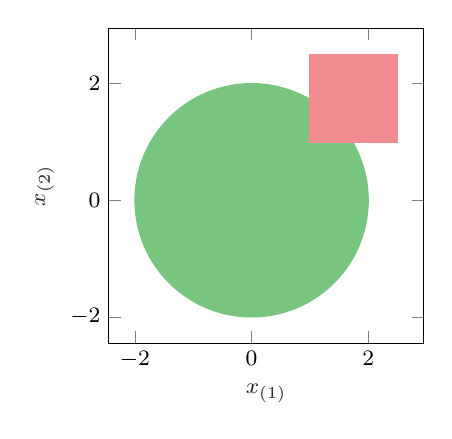
\begin{tikzpicture}
\footnotesize

\begin{axis}[%
width=4cm,
height=4cm,
at={(0in,0in)},
scale only axis,
xmin=-2.45,
xmax=2.95,
xlabel style={font=\color{white!15!black}},
xlabel={$x_{(1)}$},
ymin=-2.45,
ymax=2.95,
ylabel style={font=\color{white!15!black}},
ylabel={$x_{(2)}$},
axis background/.style={fill=white}
]

\addplot[area legend, draw=mycolor1, fill=mycolor1, forget plot]
table[row sep=crcr] {%
x	y\\
2	0.0063\\
1.9999	0.0188\\
1.9998	0.0314\\
1.9995	0.044\\
1.9992	0.0565\\
1.9988	0.0691\\
1.9983	0.0817\\
1.9978	0.0942\\
1.9971	0.1068\\
1.9964	0.1193\\
1.9956	0.1319\\
1.9948	0.1444\\
1.9928	0.1694\\
1.9917	0.182\\
1.9893	0.207\\
1.9865	0.232\\
1.985	0.2444\\
1.9818	0.2694\\
1.9782	0.2942\\
1.9763	0.3067\\
1.9744	0.3191\\
1.9702	0.3439\\
1.968	0.3562\\
1.9657	0.3686\\
1.9634	0.3809\\
1.961	0.3933\\
1.9584	0.4056\\
1.9559	0.4179\\
1.9532	0.4302\\
1.9505	0.4424\\
1.9476	0.4547\\
1.9418	0.4791\\
1.9356	0.5035\\
1.9324	0.5156\\
1.9291	0.5277\\
1.9258	0.5399\\
1.9223	0.5519\\
1.9188	0.564\\
1.9152	0.5761\\
1.9116	0.5881\\
1.9079	0.6001\\
1.904	0.6121\\
1.9002	0.624\\
1.8922	0.6478\\
1.8881	0.6597\\
1.8839	0.6716\\
1.8753	0.6952\\
1.8709	0.7069\\
1.8664	0.7187\\
1.8619	0.7304\\
1.8572	0.7421\\
1.8525	0.7537\\
1.8478	0.7654\\
1.8429	0.777\\
1.838	0.7885\\
1.833	0.8001\\
1.8279	0.8116\\
1.8228	0.823\\
1.8176	0.8345\\
1.8123	0.8459\\
1.807	0.8572\\
1.8015	0.8686\\
1.7961	0.8799\\
1.7905	0.8911\\
1.7849	0.9024\\
1.7792	0.9136\\
1.7734	0.9247\\
1.7675	0.9359\\
1.7616	0.9469\\
1.7556	0.958\\
1.7496	0.969\\
1.7435	0.98\\
1.7373	0.9909\\
1.7247	1.0127\\
1.7183	1.0235\\
1.7118	1.0343\\
1.7053	1.045\\
1.6987	1.0557\\
1.692	1.0663\\
1.6853	1.077\\
1.6785	1.0875\\
1.6647	1.1085\\
1.6577	1.119\\
1.6506	1.1294\\
1.6435	1.1397\\
1.6363	1.15\\
1.629	1.1603\\
1.6217	1.1705\\
1.6143	1.1806\\
1.6069	1.1908\\
1.5994	1.2008\\
1.5918	1.2109\\
1.5842	1.2208\\
1.5765	1.2308\\
1.5687	1.2407\\
1.5609	1.2505\\
1.553	1.2603\\
1.537	1.2797\\
1.5208	1.2989\\
1.5044	1.3179\\
1.4961	1.3273\\
1.4877	1.3367\\
1.4793	1.346\\
1.4708	1.3553\\
1.4536	1.3737\\
1.445	1.3828\\
1.4363	1.3918\\
1.4275	1.4008\\
1.4186	1.4098\\
1.4098	1.4186\\
1.4008	1.4275\\
1.3918	1.4363\\
1.3828	1.445\\
1.3737	1.4536\\
1.3553	1.4708\\
1.346	1.4793\\
1.3367	1.4877\\
1.3273	1.4961\\
1.3179	1.5044\\
1.2989	1.5208\\
1.2797	1.537\\
1.2603	1.553\\
1.2505	1.5609\\
1.2407	1.5687\\
1.2308	1.5765\\
1.2208	1.5842\\
1.2109	1.5918\\
1.2008	1.5994\\
1.1908	1.6069\\
1.1806	1.6143\\
1.1705	1.6217\\
1.1603	1.629\\
1.15	1.6363\\
1.1397	1.6435\\
1.1294	1.6506\\
1.119	1.6577\\
1.1085	1.6647\\
1.0875	1.6785\\
1.077	1.6853\\
1.0663	1.692\\
1.0557	1.6987\\
1.045	1.7053\\
1.0343	1.7118\\
1.0235	1.7183\\
1.0127	1.7247\\
0.9909	1.7373\\
0.98	1.7435\\
0.969	1.7496\\
0.958	1.7556\\
0.9469	1.7616\\
0.9359	1.7675\\
0.9247	1.7734\\
0.9136	1.7792\\
0.9024	1.7849\\
0.8911	1.7905\\
0.8799	1.7961\\
0.8686	1.8015\\
0.8572	1.807\\
0.8459	1.8123\\
0.8345	1.8176\\
0.823	1.8228\\
0.8116	1.8279\\
0.8001	1.833\\
0.7885	1.838\\
0.777	1.8429\\
0.7654	1.8478\\
0.7537	1.8525\\
0.7421	1.8572\\
0.7304	1.8619\\
0.7187	1.8664\\
0.7069	1.8709\\
0.6952	1.8753\\
0.6716	1.8839\\
0.6597	1.8881\\
0.6478	1.8922\\
0.624	1.9002\\
0.6121	1.904\\
0.6001	1.9079\\
0.5881	1.9116\\
0.5761	1.9152\\
0.564	1.9188\\
0.5519	1.9223\\
0.5399	1.9258\\
0.5277	1.9291\\
0.5156	1.9324\\
0.5035	1.9356\\
0.4791	1.9418\\
0.4547	1.9476\\
0.4424	1.9505\\
0.4302	1.9532\\
0.4179	1.9559\\
0.4056	1.9584\\
0.3933	1.961\\
0.3809	1.9634\\
0.3686	1.9657\\
0.3562	1.968\\
0.3439	1.9702\\
0.3191	1.9744\\
0.3067	1.9763\\
0.2942	1.9782\\
0.2694	1.9818\\
0.2444	1.985\\
0.232	1.9865\\
0.207	1.9893\\
0.182	1.9917\\
0.1694	1.9928\\
0.1444	1.9948\\
0.1319	1.9956\\
0.1193	1.9964\\
0.1068	1.9971\\
0.0942	1.9978\\
0.0817	1.9983\\
0.0691	1.9988\\
0.0565	1.9992\\
0.044	1.9995\\
0.0314	1.9998\\
0.0188	1.9999\\
0.0063	2\\
-0.0063	2\\
-0.0188	1.9999\\
-0.0314	1.9998\\
-0.044	1.9995\\
-0.0565	1.9992\\
-0.0691	1.9988\\
-0.0817	1.9983\\
-0.0942	1.9978\\
-0.1068	1.9971\\
-0.1193	1.9964\\
-0.1319	1.9956\\
-0.1444	1.9948\\
-0.1694	1.9928\\
-0.182	1.9917\\
-0.207	1.9893\\
-0.232	1.9865\\
-0.2444	1.985\\
-0.2694	1.9818\\
-0.2942	1.9782\\
-0.3067	1.9763\\
-0.3191	1.9744\\
-0.3439	1.9702\\
-0.3562	1.968\\
-0.3686	1.9657\\
-0.3809	1.9634\\
-0.3933	1.961\\
-0.4056	1.9584\\
-0.4179	1.9559\\
-0.4302	1.9532\\
-0.4424	1.9505\\
-0.4547	1.9476\\
-0.4791	1.9418\\
-0.5035	1.9356\\
-0.5156	1.9324\\
-0.5277	1.9291\\
-0.5399	1.9258\\
-0.5519	1.9223\\
-0.564	1.9188\\
-0.5761	1.9152\\
-0.5881	1.9116\\
-0.6001	1.9079\\
-0.6121	1.904\\
-0.624	1.9002\\
-0.6478	1.8922\\
-0.6597	1.8881\\
-0.6716	1.8839\\
-0.6952	1.8753\\
-0.7069	1.8709\\
-0.7187	1.8664\\
-0.7304	1.8619\\
-0.7421	1.8572\\
-0.7537	1.8525\\
-0.7654	1.8478\\
-0.777	1.8429\\
-0.7885	1.838\\
-0.8001	1.833\\
-0.8116	1.8279\\
-0.823	1.8228\\
-0.8345	1.8176\\
-0.8459	1.8123\\
-0.8572	1.807\\
-0.8686	1.8015\\
-0.8799	1.7961\\
-0.8911	1.7905\\
-0.9024	1.7849\\
-0.9136	1.7792\\
-0.9247	1.7734\\
-0.9359	1.7675\\
-0.9469	1.7616\\
-0.958	1.7556\\
-0.969	1.7496\\
-0.98	1.7435\\
-0.9909	1.7373\\
-1.0127	1.7247\\
-1.0235	1.7183\\
-1.0343	1.7118\\
-1.045	1.7053\\
-1.0557	1.6987\\
-1.0663	1.692\\
-1.077	1.6853\\
-1.0875	1.6785\\
-1.1085	1.6647\\
-1.119	1.6577\\
-1.1294	1.6506\\
-1.1397	1.6435\\
-1.15	1.6363\\
-1.1603	1.629\\
-1.1705	1.6217\\
-1.1806	1.6143\\
-1.1908	1.6069\\
-1.2008	1.5994\\
-1.2109	1.5918\\
-1.2208	1.5842\\
-1.2308	1.5765\\
-1.2407	1.5687\\
-1.2505	1.5609\\
-1.2603	1.553\\
-1.2797	1.537\\
-1.2989	1.5208\\
-1.3179	1.5044\\
-1.3273	1.4961\\
-1.3367	1.4877\\
-1.346	1.4793\\
-1.3553	1.4708\\
-1.3737	1.4536\\
-1.3828	1.445\\
-1.3918	1.4363\\
-1.4008	1.4275\\
-1.4098	1.4186\\
-1.4186	1.4098\\
-1.4275	1.4008\\
-1.4363	1.3918\\
-1.445	1.3828\\
-1.4536	1.3737\\
-1.4708	1.3553\\
-1.4793	1.346\\
-1.4877	1.3367\\
-1.4961	1.3273\\
-1.5044	1.3179\\
-1.5208	1.2989\\
-1.537	1.2797\\
-1.553	1.2603\\
-1.5609	1.2505\\
-1.5687	1.2407\\
-1.5765	1.2308\\
-1.5842	1.2208\\
-1.5918	1.2109\\
-1.5994	1.2008\\
-1.6069	1.1908\\
-1.6143	1.1806\\
-1.6217	1.1705\\
-1.629	1.1603\\
-1.6363	1.15\\
-1.6435	1.1397\\
-1.6506	1.1294\\
-1.6577	1.119\\
-1.6647	1.1085\\
-1.6785	1.0875\\
-1.6853	1.077\\
-1.692	1.0663\\
-1.6987	1.0557\\
-1.7053	1.045\\
-1.7118	1.0343\\
-1.7183	1.0235\\
-1.7247	1.0127\\
-1.7373	0.9909\\
-1.7435	0.98\\
-1.7496	0.969\\
-1.7556	0.958\\
-1.7616	0.9469\\
-1.7675	0.9359\\
-1.7734	0.9247\\
-1.7792	0.9136\\
-1.7849	0.9024\\
-1.7905	0.8911\\
-1.7961	0.8799\\
-1.8015	0.8686\\
-1.807	0.8572\\
-1.8123	0.8459\\
-1.8176	0.8345\\
-1.8228	0.823\\
-1.8279	0.8116\\
-1.833	0.8001\\
-1.838	0.7885\\
-1.8429	0.777\\
-1.8478	0.7654\\
-1.8525	0.7537\\
-1.8572	0.7421\\
-1.8619	0.7304\\
-1.8664	0.7187\\
-1.8709	0.7069\\
-1.8753	0.6952\\
-1.8839	0.6716\\
-1.8881	0.6597\\
-1.8922	0.6478\\
-1.9002	0.624\\
-1.904	0.6121\\
-1.9079	0.6001\\
-1.9116	0.5881\\
-1.9152	0.5761\\
-1.9188	0.564\\
-1.9223	0.5519\\
-1.9258	0.5399\\
-1.9291	0.5277\\
-1.9324	0.5156\\
-1.9356	0.5035\\
-1.9418	0.4791\\
-1.9476	0.4547\\
-1.9505	0.4424\\
-1.9532	0.4302\\
-1.9559	0.4179\\
-1.9584	0.4056\\
-1.961	0.3933\\
-1.9634	0.3809\\
-1.9657	0.3686\\
-1.968	0.3562\\
-1.9702	0.3439\\
-1.9744	0.3191\\
-1.9763	0.3067\\
-1.9782	0.2942\\
-1.9818	0.2694\\
-1.985	0.2444\\
-1.9865	0.232\\
-1.9893	0.207\\
-1.9917	0.182\\
-1.9928	0.1694\\
-1.9948	0.1444\\
-1.9956	0.1319\\
-1.9964	0.1193\\
-1.9971	0.1068\\
-1.9978	0.0942\\
-1.9983	0.0817\\
-1.9988	0.0691\\
-1.9992	0.0565\\
-1.9995	0.044\\
-1.9998	0.0314\\
-1.9999	0.0188\\
-2	0.0063\\
-2	-0.0063\\
-1.9999	-0.0188\\
-1.9998	-0.0314\\
-1.9995	-0.044\\
-1.9992	-0.0565\\
-1.9988	-0.0691\\
-1.9983	-0.0817\\
-1.9978	-0.0942\\
-1.9971	-0.1068\\
-1.9964	-0.1193\\
-1.9956	-0.1319\\
-1.9948	-0.1444\\
-1.9928	-0.1694\\
-1.9917	-0.182\\
-1.9893	-0.207\\
-1.9865	-0.232\\
-1.985	-0.2444\\
-1.9818	-0.2694\\
-1.9782	-0.2942\\
-1.9763	-0.3067\\
-1.9744	-0.3191\\
-1.9702	-0.3439\\
-1.968	-0.3562\\
-1.9657	-0.3686\\
-1.9634	-0.3809\\
-1.961	-0.3933\\
-1.9584	-0.4056\\
-1.9559	-0.4179\\
-1.9532	-0.4302\\
-1.9505	-0.4424\\
-1.9476	-0.4547\\
-1.9418	-0.4791\\
-1.9356	-0.5035\\
-1.9324	-0.5156\\
-1.9291	-0.5277\\
-1.9258	-0.5399\\
-1.9223	-0.5519\\
-1.9188	-0.564\\
-1.9152	-0.5761\\
-1.9116	-0.5881\\
-1.9079	-0.6001\\
-1.904	-0.6121\\
-1.9002	-0.624\\
-1.8922	-0.6478\\
-1.8881	-0.6597\\
-1.8839	-0.6716\\
-1.8753	-0.6952\\
-1.8709	-0.7069\\
-1.8664	-0.7187\\
-1.8619	-0.7304\\
-1.8572	-0.7421\\
-1.8525	-0.7537\\
-1.8478	-0.7654\\
-1.8429	-0.777\\
-1.838	-0.7885\\
-1.833	-0.8001\\
-1.8279	-0.8116\\
-1.8228	-0.823\\
-1.8176	-0.8345\\
-1.8123	-0.8459\\
-1.807	-0.8572\\
-1.8015	-0.8686\\
-1.7961	-0.8799\\
-1.7905	-0.8911\\
-1.7849	-0.9024\\
-1.7792	-0.9136\\
-1.7734	-0.9247\\
-1.7675	-0.9359\\
-1.7616	-0.9469\\
-1.7556	-0.958\\
-1.7496	-0.969\\
-1.7435	-0.98\\
-1.7373	-0.9909\\
-1.7247	-1.0127\\
-1.7183	-1.0235\\
-1.7118	-1.0343\\
-1.7053	-1.045\\
-1.6987	-1.0557\\
-1.692	-1.0663\\
-1.6853	-1.077\\
-1.6785	-1.0875\\
-1.6647	-1.1085\\
-1.6577	-1.119\\
-1.6506	-1.1294\\
-1.6435	-1.1397\\
-1.6363	-1.15\\
-1.629	-1.1603\\
-1.6217	-1.1705\\
-1.6143	-1.1806\\
-1.6069	-1.1908\\
-1.5994	-1.2008\\
-1.5918	-1.2109\\
-1.5842	-1.2208\\
-1.5765	-1.2308\\
-1.5687	-1.2407\\
-1.5609	-1.2505\\
-1.553	-1.2603\\
-1.537	-1.2797\\
-1.5208	-1.2989\\
-1.5044	-1.3179\\
-1.4961	-1.3273\\
-1.4877	-1.3367\\
-1.4793	-1.346\\
-1.4708	-1.3553\\
-1.4536	-1.3737\\
-1.445	-1.3828\\
-1.4363	-1.3918\\
-1.4275	-1.4008\\
-1.4186	-1.4098\\
-1.4098	-1.4186\\
-1.4008	-1.4275\\
-1.3918	-1.4363\\
-1.3828	-1.445\\
-1.3737	-1.4536\\
-1.3553	-1.4708\\
-1.346	-1.4793\\
-1.3367	-1.4877\\
-1.3273	-1.4961\\
-1.3179	-1.5044\\
-1.2989	-1.5208\\
-1.2797	-1.537\\
-1.2603	-1.553\\
-1.2505	-1.5609\\
-1.2407	-1.5687\\
-1.2308	-1.5765\\
-1.2208	-1.5842\\
-1.2109	-1.5918\\
-1.2008	-1.5994\\
-1.1908	-1.6069\\
-1.1806	-1.6143\\
-1.1705	-1.6217\\
-1.1603	-1.629\\
-1.15	-1.6363\\
-1.1397	-1.6435\\
-1.1294	-1.6506\\
-1.119	-1.6577\\
-1.1085	-1.6647\\
-1.0875	-1.6785\\
-1.077	-1.6853\\
-1.0663	-1.692\\
-1.0557	-1.6987\\
-1.045	-1.7053\\
-1.0343	-1.7118\\
-1.0235	-1.7183\\
-1.0127	-1.7247\\
-0.9909	-1.7373\\
-0.98	-1.7435\\
-0.969	-1.7496\\
-0.958	-1.7556\\
-0.9469	-1.7616\\
-0.9359	-1.7675\\
-0.9247	-1.7734\\
-0.9136	-1.7792\\
-0.9024	-1.7849\\
-0.8911	-1.7905\\
-0.8799	-1.7961\\
-0.8686	-1.8015\\
-0.8572	-1.807\\
-0.8459	-1.8123\\
-0.8345	-1.8176\\
-0.823	-1.8228\\
-0.8116	-1.8279\\
-0.8001	-1.833\\
-0.7885	-1.838\\
-0.777	-1.8429\\
-0.7654	-1.8478\\
-0.7537	-1.8525\\
-0.7421	-1.8572\\
-0.7304	-1.8619\\
-0.7187	-1.8664\\
-0.7069	-1.8709\\
-0.6952	-1.8753\\
-0.6716	-1.8839\\
-0.6597	-1.8881\\
-0.6478	-1.8922\\
-0.624	-1.9002\\
-0.6121	-1.904\\
-0.6001	-1.9079\\
-0.5881	-1.9116\\
-0.5761	-1.9152\\
-0.564	-1.9188\\
-0.5519	-1.9223\\
-0.5399	-1.9258\\
-0.5277	-1.9291\\
-0.5156	-1.9324\\
-0.5035	-1.9356\\
-0.4791	-1.9418\\
-0.4547	-1.9476\\
-0.4424	-1.9505\\
-0.4302	-1.9532\\
-0.4179	-1.9559\\
-0.4056	-1.9584\\
-0.3933	-1.961\\
-0.3809	-1.9634\\
-0.3686	-1.9657\\
-0.3562	-1.968\\
-0.3439	-1.9702\\
-0.3191	-1.9744\\
-0.3067	-1.9763\\
-0.2942	-1.9782\\
-0.2694	-1.9818\\
-0.2444	-1.985\\
-0.232	-1.9865\\
-0.207	-1.9893\\
-0.182	-1.9917\\
-0.1694	-1.9928\\
-0.1444	-1.9948\\
-0.1319	-1.9956\\
-0.1193	-1.9964\\
-0.1068	-1.9971\\
-0.0942	-1.9978\\
-0.0817	-1.9983\\
-0.0691	-1.9988\\
-0.0565	-1.9992\\
-0.044	-1.9995\\
-0.0314	-1.9998\\
-0.0188	-1.9999\\
-0.0063	-2\\
0.0063	-2\\
0.0188	-1.9999\\
0.0314	-1.9998\\
0.044	-1.9995\\
0.0565	-1.9992\\
0.0691	-1.9988\\
0.0817	-1.9983\\
0.0942	-1.9978\\
0.1068	-1.9971\\
0.1193	-1.9964\\
0.1319	-1.9956\\
0.1444	-1.9948\\
0.1694	-1.9928\\
0.182	-1.9917\\
0.207	-1.9893\\
0.232	-1.9865\\
0.2444	-1.985\\
0.2694	-1.9818\\
0.2942	-1.9782\\
0.3067	-1.9763\\
0.3191	-1.9744\\
0.3439	-1.9702\\
0.3562	-1.968\\
0.3686	-1.9657\\
0.3809	-1.9634\\
0.3933	-1.961\\
0.4056	-1.9584\\
0.4179	-1.9559\\
0.4302	-1.9532\\
0.4424	-1.9505\\
0.4547	-1.9476\\
0.4791	-1.9418\\
0.5035	-1.9356\\
0.5156	-1.9324\\
0.5277	-1.9291\\
0.5399	-1.9258\\
0.5519	-1.9223\\
0.564	-1.9188\\
0.5761	-1.9152\\
0.5881	-1.9116\\
0.6001	-1.9079\\
0.6121	-1.904\\
0.624	-1.9002\\
0.6478	-1.8922\\
0.6597	-1.8881\\
0.6716	-1.8839\\
0.6952	-1.8753\\
0.7069	-1.8709\\
0.7187	-1.8664\\
0.7304	-1.8619\\
0.7421	-1.8572\\
0.7537	-1.8525\\
0.7654	-1.8478\\
0.777	-1.8429\\
0.7885	-1.838\\
0.8001	-1.833\\
0.8116	-1.8279\\
0.823	-1.8228\\
0.8345	-1.8176\\
0.8459	-1.8123\\
0.8572	-1.807\\
0.8686	-1.8015\\
0.8799	-1.7961\\
0.8911	-1.7905\\
0.9024	-1.7849\\
0.9136	-1.7792\\
0.9247	-1.7734\\
0.9359	-1.7675\\
0.9469	-1.7616\\
0.958	-1.7556\\
0.969	-1.7496\\
0.98	-1.7435\\
0.9909	-1.7373\\
1.0127	-1.7247\\
1.0235	-1.7183\\
1.0343	-1.7118\\
1.045	-1.7053\\
1.0557	-1.6987\\
1.0663	-1.692\\
1.077	-1.6853\\
1.0875	-1.6785\\
1.1085	-1.6647\\
1.119	-1.6577\\
1.1294	-1.6506\\
1.1397	-1.6435\\
1.15	-1.6363\\
1.1603	-1.629\\
1.1705	-1.6217\\
1.1806	-1.6143\\
1.1908	-1.6069\\
1.2008	-1.5994\\
1.2109	-1.5918\\
1.2208	-1.5842\\
1.2308	-1.5765\\
1.2407	-1.5687\\
1.2505	-1.5609\\
1.2603	-1.553\\
1.2797	-1.537\\
1.2989	-1.5208\\
1.3179	-1.5044\\
1.3273	-1.4961\\
1.3367	-1.4877\\
1.346	-1.4793\\
1.3553	-1.4708\\
1.3737	-1.4536\\
1.3828	-1.445\\
1.3918	-1.4363\\
1.4008	-1.4275\\
1.4098	-1.4186\\
1.4186	-1.4098\\
1.4275	-1.4008\\
1.4363	-1.3918\\
1.445	-1.3828\\
1.4536	-1.3737\\
1.4708	-1.3553\\
1.4793	-1.346\\
1.4877	-1.3367\\
1.4961	-1.3273\\
1.5044	-1.3179\\
1.5208	-1.2989\\
1.537	-1.2797\\
1.553	-1.2603\\
1.5609	-1.2505\\
1.5687	-1.2407\\
1.5765	-1.2308\\
1.5842	-1.2208\\
1.5918	-1.2109\\
1.5994	-1.2008\\
1.6069	-1.1908\\
1.6143	-1.1806\\
1.6217	-1.1705\\
1.629	-1.1603\\
1.6363	-1.15\\
1.6435	-1.1397\\
1.6506	-1.1294\\
1.6577	-1.119\\
1.6647	-1.1085\\
1.6785	-1.0875\\
1.6853	-1.077\\
1.692	-1.0663\\
1.6987	-1.0557\\
1.7053	-1.045\\
1.7118	-1.0343\\
1.7183	-1.0235\\
1.7247	-1.0127\\
1.7373	-0.9909\\
1.7435	-0.98\\
1.7496	-0.969\\
1.7556	-0.958\\
1.7616	-0.9469\\
1.7675	-0.9359\\
1.7734	-0.9247\\
1.7792	-0.9136\\
1.7849	-0.9024\\
1.7905	-0.8911\\
1.7961	-0.8799\\
1.8015	-0.8686\\
1.807	-0.8572\\
1.8123	-0.8459\\
1.8176	-0.8345\\
1.8228	-0.823\\
1.8279	-0.8116\\
1.833	-0.8001\\
1.838	-0.7885\\
1.8429	-0.777\\
1.8478	-0.7654\\
1.8525	-0.7537\\
1.8572	-0.7421\\
1.8619	-0.7304\\
1.8664	-0.7187\\
1.8709	-0.7069\\
1.8753	-0.6952\\
1.8839	-0.6716\\
1.8881	-0.6597\\
1.8922	-0.6478\\
1.9002	-0.624\\
1.904	-0.6121\\
1.9079	-0.6001\\
1.9116	-0.5881\\
1.9152	-0.5761\\
1.9188	-0.564\\
1.9223	-0.5519\\
1.9258	-0.5399\\
1.9291	-0.5277\\
1.9324	-0.5156\\
1.9356	-0.5035\\
1.9418	-0.4791\\
1.9476	-0.4547\\
1.9505	-0.4424\\
1.9532	-0.4302\\
1.9559	-0.4179\\
1.9584	-0.4056\\
1.961	-0.3933\\
1.9634	-0.3809\\
1.9657	-0.3686\\
1.968	-0.3562\\
1.9702	-0.3439\\
1.9744	-0.3191\\
1.9763	-0.3067\\
1.9782	-0.2942\\
1.9818	-0.2694\\
1.985	-0.2444\\
1.9865	-0.232\\
1.9893	-0.207\\
1.9917	-0.182\\
1.9928	-0.1694\\
1.9948	-0.1444\\
1.9956	-0.1319\\
1.9964	-0.1193\\
1.9971	-0.1068\\
1.9978	-0.0942\\
1.9983	-0.0817\\
1.9988	-0.0691\\
1.9992	-0.0565\\
1.9995	-0.044\\
1.9998	-0.0314\\
1.9999	-0.0188\\
2	-0.0063\\
2	0.0063\\
}--cycle;

\addplot[area legend, draw=mycolor2, fill=mycolor2, forget plot]
table[row sep=crcr] {%
x	y\\
1	1\\
2.5	1\\
2.5	2.5\\
1	2.5\\
1	1\\
}--cycle;
\end{axis}
\end{tikzpicture}%
\end{minipage}
\begin{minipage}[t]{0.3\textwidth}
	\vspace{0pt}
	\centering
	\includetikz{./figures/tikz/add-functionality/example_specification}
\end{minipage}
\end{center}

Next, we explain the methods of class \texttt{specification} in detail.

\subsubsection{add}
\label{sec:specAdd}

The method \texttt{add} unites two specifications:
\begin{equation*}
	\texttt{spec} = \texttt{add}(\texttt{spec1},\texttt{spec2}),
\end{equation*}
where \texttt{spec1} and \texttt{spec2} are both objects of class \texttt{specification}. The specifications defined by \texttt{spec1} and \texttt{spec2} both have to be satisfied for the resulting specification \texttt{spec} to be satisfied.

\subsubsection{check}

The method \texttt{check} checks if a set $\mathcal{S} \subset \Rn$ satisfies the specification defined by the object \texttt{spec} of class \texttt{specification}:

\begin{equation*}
	\texttt{res} = \texttt{check}(\texttt{spec},\mathcal{S}),
\end{equation*}
where \texttt{res} is \texttt{true} if the specification is satisfied, and \texttt{false} otherwise.
